\documentclass[final,hyperref={pdfpagelabels=false}]{beamer}
\usepackage{grffile}
\mode<presentation>{\usetheme{NIPS}}
\usepackage[english]{babel}
\usepackage[latin1]{inputenc}
\usepackage{amsmath,amsthm, amssymb, latexsym}
\usepackage{graphicx}
\usepackage{subfigure}
\usepackage{tikz}
\usetikzlibrary{arrows,backgrounds,fit,petri,positioning,shapes}
%\usefonttheme[onlymath]{serif}
\boldmath
%\usepackage[orientation=portrait,size=a0,scale=1.4,debug]{beamerposter}
\usepackage[size=custom,width=88.9,height=132.08,scale=1.4,debug]{beamerposter}
% change list indention level
% \setdefaultleftmargin{3em}{}{}{}{}{}


%\usepackage{snapshot} % will write a .dep file with all dependencies, allows for easy bundling

\usepackage{array,booktabs,tabularx}
\newcolumntype{Z}{>{\centering\arraybackslash}X} % centered tabularx columns
\newcommand{\pphantom}{\textcolor{ta3aluminium}} % phantom introduces a vertical space in p formatted table columns??!!

\listfiles
\providecommand\thispdfpagelabel[1]{}

%%%%%%%%%%%%%%%%%%%%%%%%%%%%%%%%%%%%%%%%%%%%%%%%%%%%%%%%%%%%%%%%%%%%%%%%%%%%%%%%%%%%%%
\graphicspath{{figures/}}

\newcommand{\reals}{\mathbb{R}}
\newcommand{\trans}{\mathrm{T}}

\DeclareMathOperator{\Tr}{Tr}
\DeclareMathOperator*{\argmax}{argmax}
\DeclareMathOperator*{\argmin}{argmin}
\DeclareMathOperator{\diag}{diag}
\DeclareMathOperator{\rank}{rank}
\newcommand{\Normal}[1][]{\mathcal{N}_{#1}}
\newcommand{\Wishart}[1][]{\mathcal{W}_{#1}}

\newcommand{\prob}{\mathbb{P}}
\newcommand{\E}{\mathbb{E}}
\DeclareMathOperator{\RSS}{RSS}

\newtheorem{proposition}[theorem]{Proposition}
\newtheorem{remark}[theorem]{Remark}


\title{\huge Regularized Laplacian Estimation and \\ Fast Eigenvector
Approximation}
\author{Patrick O. Perry and Michael W. Mahoney}
\institute{NYU Stern and Stanford University}
%\date[Sep. 8th, 2009]{Sep. 8th, 2009}

%%%%%%%%%%%%%%%%%%%%%%%%%%%%%%%%%%%%%%%%%%%%%%%%%%%%%%%%%%%%%%%%%%%%%%%%%%%%%%%%%%%%%%
\newlength{\columnheight}
\setlength{\columnheight}{120cm}


%%%%%%%%%%%%%%%%%%%%%%%%%%%%%%%%%%%%%%%%%%%%%%%%%%%%%%%%%%%%%%%%%%%%%%%%%%%%%%%%%%%%%%
\begin{document}
\begin{frame}
  \begin{columns}
    % ---------------------------------------------------------%
    % Set up a column 
    \begin{column}{.49\textwidth}
      \begin{beamercolorbox}[center,wd=\textwidth]{postercolumn}
        \begin{minipage}[T]{.95\textwidth}  % tweaks the width, makes a new \textwidth
          \parbox[t][\columnheight]{\textwidth}{ % must be some better way to set the the height, width and textwidth simultaneously
            % Since all columns are the same length, it is all nice and tidy.  You have to get the height empirically
            % ---------------------------------------------------------%
            % fill each column with content            
            \begin{block}{Structure in high-dimensional data}
              \begin{itemize}

              \item Eigenvectors reveal structure
	        \begin{description}
	      	\item[Graph Laplacian] spectral clustering
		\item[Covariance matrix] factor analysis
		\item[Modularity matrix] community detection
		\end{description}

		\vspace{1em}
              \item Diffusions reveal structure
	        \begin{description}
		\item[Heat diffusion] evolution determined by heat equation
		\item[PageRank surfer] random walk with teleportation
		\item[Truncated random walk] finite-length random walk
		\end{description}

              \end{itemize}              

		\vspace{1em}
	      One way to find structure in a high-dimensional dataset is by
	      examining the eigenstructures of certain matrices related to the
	      data; another way is by distributing charge (randomly,
	      adversarially, etc.) on the data points and letting the
	      distribution of the charge evolve according to a diffusion.

            \end{block}

            \vfill

            \begin{block}{Three eigenvector problems for graph Laplacian $L$}
	    \begin{itemize}
	      \item Consider three structure-revealing eigenvector problems for a
	      (normalized) graph Laplacian:

              \begin{itemize}
              \item Original: minimize $x' L x$
              \item Relaxed to an SDP: minimize $\mathrm{Tr}(L X)$
              \item Regularized: minimize $\mathrm{Tr}(L X) + \tfrac{1}{\eta} G(X)$
              \end{itemize}
	      \end{itemize}

	      \vspace{1em}
	      Mahoney and Orechhia (2011) show that certain choices of the penalty
	      function $G(X)$ result in the solutions of the regularized
	      eigenenvector problem; equivalently, running certain
	      diffusion-based procedures \emph{implicitly} solves a
	      regularized SDP \emph{exactly}.  The choice of $1/\eta$ is
	      related to the parameters of the diffusion.

\begin{center}
    \begin{tabular}{ccc}
      $G(X)$ &\phantom{MMM} & Solution \\
      \hline
      $\mathrm{Tr}(X \log X) - \mathrm{Tr}(X)$ && Heat Kernel \\
      $- \log |X|$ && PageRank  \\
      $\mathrm{Tr}(X^k)$ && Lazy Random Walk
    \end{tabular}
\end{center}
	      
            \end{block}

	    \vfill

            \begin{block}{Regularization}
	      \begin{itemize}
	        \item In \emph{explicit} regularization, we add a ``penalty'' to the
		optimization criterion.

		\vspace{1em}
		\item \textbf{Question:} Can regularization be implemented
		\emph{implicitly} by running fast approximation algorithms, rather
		than explicitly solving a modified problem exactly?
		\begin{itemize}
		\item Leskovec, Lang, and Mahoney (2010) empirically observed
		implicit regularization for spectral-based versus flow-based
		approximation algorithms for graph partitioning.

		\item Mahoney and Orecchia (2011) theoretically proved that
		certain diffusion-based approximation algorithms implicitly solve
		regularized versions of the exact algorithm.
		\end{itemize}

		\vspace{1em}
		\item \textbf{Question:} Is there a theoretical basis for
		which dynamics (Heat Kernel, PageRank, or Lazy Random Walk) are appropriate
		for which classes of graphs?

		\begin{itemize}
		\item We can answer this question by filling in the missing
		link:
	    \begin{center}
	    \begin{tikzpicture}[scale=2]
	 \matrix[nodes={draw, ultra thick, fill=blue!20, minimum width=6em, minimum height=4em},
        row sep=1em,column sep=3em,ampersand replacement=\&] {
      \node[ellipse] (graphs) {Graphs};\&
      \node[ellipse] (regularization) {Regularization};\&
      \node[ellipse] (structure) {$\stackrel{\hbox{Diffusion/}}{\hbox{Structure}}$};\\
    };
    \path[<->, ultra thick]
      (regularization)
        edge node[auto, rotate=45, anchor=south west] {MO (2011)}
          (structure)
      (graphs)
        edge [bend right=30] node[below] {Empirical experience}
          (structure);
    \path[<->, ultra thick, dashed]
      (graphs)
        edge node[above, rotate=45, anchor=south west] {???}
          (regularization);
\end{tikzpicture}
\end{center}
\end{itemize}
\end{itemize}
	    \end{block}

            \vfill


            \vfill
            \begin{block}{Analogy to linear regression: regularization as ``Bayesianization''}
  \begin{itemize}
    \item Observe $n$ predictor-response pairs in $\mathbb{R}^p \times \mathbb{R}$:
      $(x_1, y_1), \dotsc, (x_n, y_n)$
    \item Original problem: find $\beta$ to minimize $F(\beta) =
    \sum_i \|y_i - \beta' x_i \|_2^2$
    \item Regularized: minimize $F(\beta) + \frac{1}{\eta} \| \beta \|_2^2$
    (ridge) or $F(\beta) + \frac{1}{\eta} \| \beta \|_1$ (lasso)
    \item Bayesian formulation:
    \end{itemize}
    \vspace{1em}

\begin{center}
  \begin{tikzpicture}
    [pre/.style={<-, >=stealth', semithick},
     post/.style={->, >=stealth', semithick},
     py/.style={color=blue},
     pbeta/.style={color=red},
     scale=0.75, transform shape]

    \node (model)
      {$y_i | x_i, \beta \sim \mathrm{Normal}(x_i' \beta, \sigma^2)$} ;
    \node (likelihood) [py, below=of model, yshift=1cm]
      {$\exp\{ -\frac{1}{2 \sigma^2} \sum_i (y_i - \beta' x_i)^2\}$};

    \node (normal)  [below left=of likelihood, xshift=2.5cm]
      {$\beta_j \sim \mathrm{Normal}(0, \tau^2)$};
    \node (normal prior) [pbeta, below=of normal, yshift=1cm]
      {$\exp\{ -\frac{1}{2 \tau^2} \|\beta\|_2^2 \}$};

    \node (laplace) [below right=of likelihood, xshift=-2.5cm]
      {$\beta_j \sim \mathrm{Laplace}(\mu)$};
    \node (laplace prior) [pbeta, below=of laplace, yshift=1cm]
      {$\exp\{ -\frac{1}{\mu} \|\beta\|_1 \}$};

    \node (tee) [circle, at= (model |- normal), yshift=1cm, inner sep=0,
                 fill=black, minimum size=0.5pt, draw] {}
      edge[pre] (likelihood)
      edge[post] (normal)
      edge[post] (laplace);

    \node (l2) [below=of normal prior]  {$\ell_2$-regularized LS}
      edge[pre] (normal prior);
    \node (l1) [below=of laplace prior] {$\ell_1$-regularized LS}
      edge[pre] (laplace prior);

    \node (prior label) [left=of normal]                    {Prior};
    \node (pbeta label) [pbeta, at=(prior label |- normal prior)]  {$p(\beta)$};
    \node (model label) [at=(prior label |- model)]         {Model};
    \node (py label)    [py, at=(prior label |- likelihood)]    {$p(y | \beta)$};
    \node (map label)   [at=(prior label |- l2), align=center] {MAP\\ Estimate};
  \end{tikzpicture}
  \end{center}

  \vspace{2em}
  Regularization is equivalent to ``Bayesianization'' in the sense that
  the solution to the regularized problem is equal to the maximim \textit{a posteriori} probability
  (MAP) estimate of the parameter with a prior determined by the
  regularization penalty.

	    
            \end{block}
          }
        \end{minipage}
      \end{beamercolorbox}
    \end{column}
    % ---------------------------------------------------------%
    % end the column

    % ---------------------------------------------------------%
    % Set up a column 
    \begin{column}{.49\textwidth}
      \begin{beamercolorbox}[center,wd=\textwidth]{postercolumn}
        \begin{minipage}[T]{.95\textwidth} % tweaks the width, makes a new \textwidth
          \parbox[t][\columnheight]{\textwidth}{ % must be some better way to set the the height, width and textwidth simultaneously
            % Since all columns are the same length, it is all nice and tidy.  You have to get the height empirically
            % ---------------------------------------------------------%
            % fill each column with content
            
            \begin{block}{Bayesian inference for the population Laplacian (broadly)}
  \begin{itemize}
    \item population Laplacian, $\mathcal{L}$ from prior $p(\mathcal{L})$
    \item observed (sample) Laplacian from distribution $p(L \mid \mathcal{L})$
    \item estimate $\mathcal{\hat L} = \argmax_{\mathcal{L}} \{ p(\mathcal{L} \mid L) \}$
    \item equivalently,
      $\mathcal{\hat L} = \argmin_{\mathcal{L}} \{ -\log p(L \mid \mathcal{L}) -\log p(\mathcal{L}) \}$
  \end{itemize}

  \vspace{1em}

  To apply the Bayesian formalism to the Laplacian eigenvector problem, we
assume that there exists a ``population'' Laplacian $\mathcal{L}$; we construe
the observed (sample) Laplacian as a noisy version of $\mathcal{L}$.  In
estimating $\mathcal{L}$, the negative log of the likelihood plays the role of
the optimization criterion; the negative log of the prior distribution for
$\mathcal{L}$ plays the role of the penalty function.
  
            \end{block}

            \vfill
            \begin{block}{Bayesian inference for the population Laplacian (specifics)}
	    \begin{itemize}
	      \item If the prior $p(\mathcal{L})$ is orthogonally-invariant and the
	        eigenvalues of $\Theta = [\Tr(\mathcal{L}^+)]^{-1} \mathcal{L}^{+}$
		are exchangeable and neutral\ldots

	      \item \ldots and $p(L\mid \mathcal{L})$ is the density of
	      $\frac{1}{m} \mathrm{Wishart}(\mathcal{L}, m)$

	      \item \ldots then $\mathcal{\hat L}$, the MAP estimate of
	      $\mathcal{L}$, is such that $\hat \Theta$ solves the
	      Mahoney-Orecchia regularized SDP with $G(X) = -\log |X|$ and
	      $\eta$ given by
	      \[
		\eta = \frac{m \hat \tau}{m + 2 (\alpha - 1)},
	      \]
	      where $\hat \tau = \mathrm{Tr}(\mathcal{\hat L}^+)$,
	      $\hat \Theta = \hat \tau^{-1} \mathcal{\hat L}^+$,
	      and $\alpha$ is prior's shape parameter.  This is the SDP
	      whose solution is the PageRank diffusion.
	    \end{itemize}
	    \vspace{1em}
	    For graphs with properties similar to the above model, PageRank
	    diffusions are natural estimators of population structure.
	    Note: with different choices of priors, one can recover the Heat
	    Kernel and Random Walk solutions.
            \end{block}

            \vfill

            \begin{block}{Empirical setup}
	    \begin{itemize}
	    \item We generate a population Laplacian $\mathcal{L}$ by
	    performing $s$ edge swaps strting from a 2-dimensional grid with
	    $\mu$ edges.
	    \end{itemize}

  \begin{center}
  \makebox{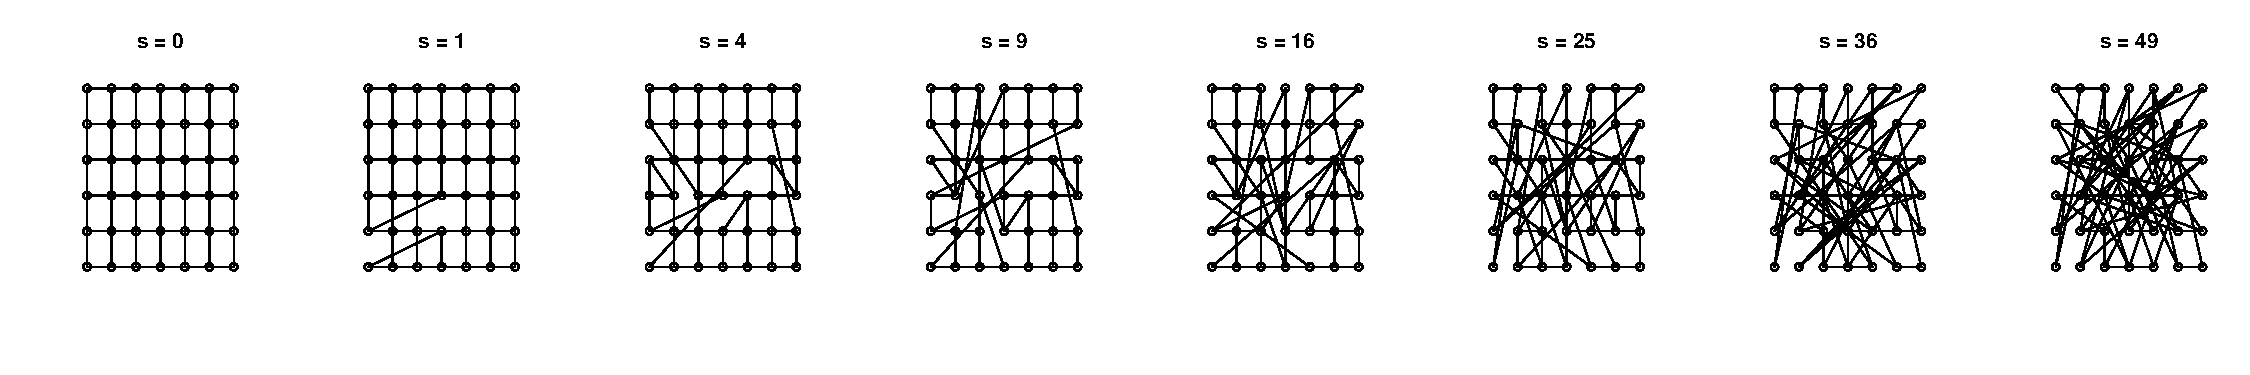
\includegraphics[scale=1.0]{plots/interpolate-graphs-long}}
  \end{center}
  \vspace{-1em}
  When $s = 0$ the population graph with Laplacian $\mathcal{L}$ is a
  low-dimensional grid; as $s \to \infty$, it becomes an expander-like 
  random graph.
  \vspace{1em}

	    \begin{itemize}
  \item Given a population graph with Laplacian $\mathcal{L}$,
  we generate a sample Laplacian $L$ by sampling $m$ edges.
  In the estimation experiment, we get to observe $L$ but not $\mathcal{L}$.
	    \end{itemize}

  \begin{center}
  \makebox{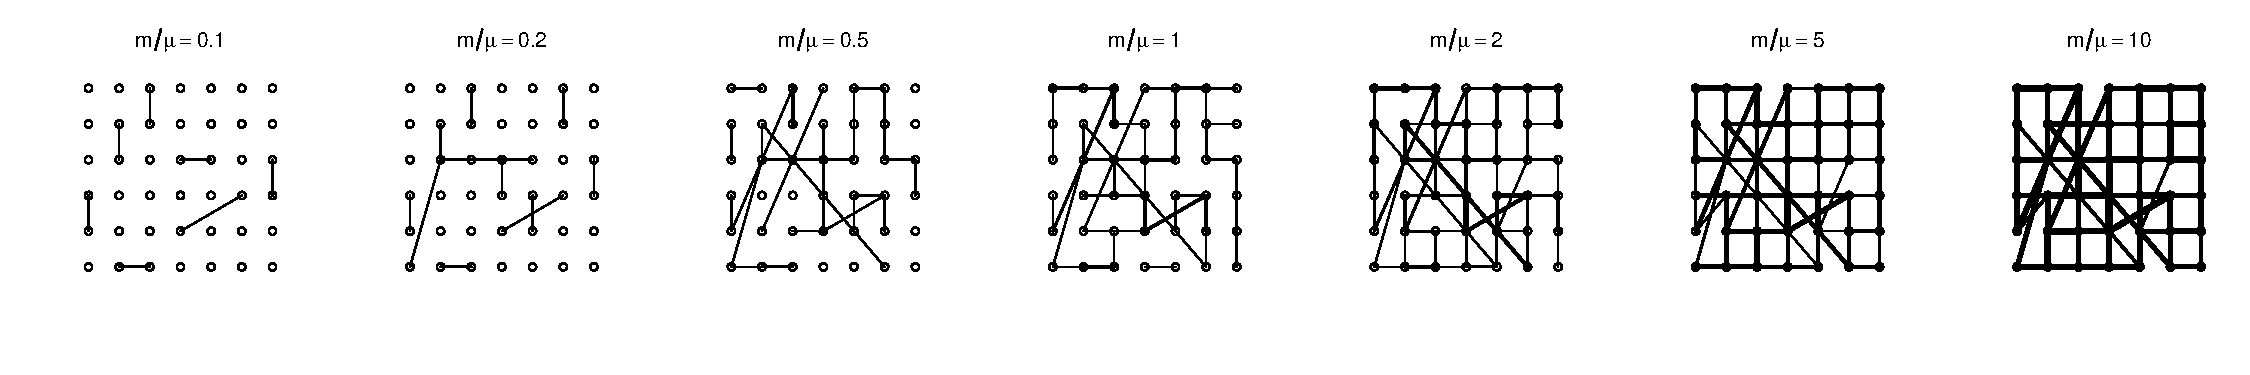
\includegraphics[scale=1.0]{plots/sample-graphs-long}}
  \end{center}
  \vspace{-1em}

  As $m / \mu$ increases, the sample Laplacian $L$ approaches the
  population $\mathcal{L}$.

%\vspace{1em}
  %\begin{itemize}
  %\item This \emph{approximates} the theoretical model.
  %\end{itemize}
  
	    \end{block}

	    \vfill

            \begin{block}{Empirical evaluation}
\begin{columns}
  \begin{column}{.25\textwidth}
    \begin{center}
    {\tiny Eigenvalues of $\Theta = (\Tr(\mathcal{L^+}))^{-1} \mathcal{L^+}$}
    \vspace{-0.5em}

    \makebox{\label{F:interpolate}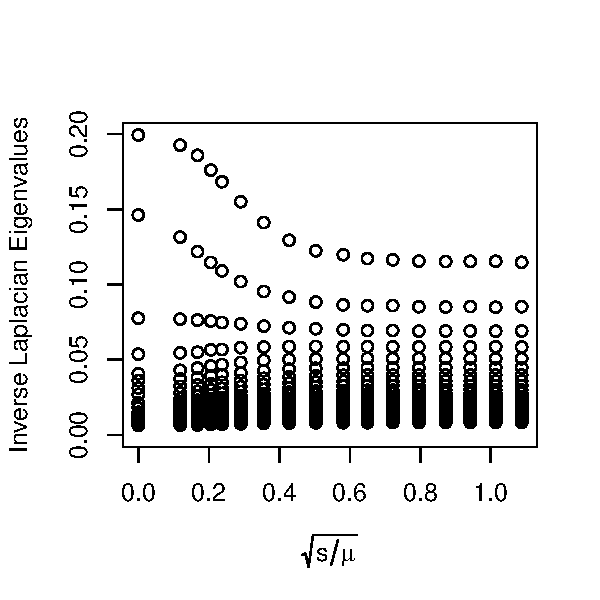
\includegraphics[scale=0.5]{plots/interpolate}}
      
    {\tiny Eigenvalues of model prior with shape $\alpha$}
    \vspace{-0.5em}

    \makebox{\label{F:dirichlet}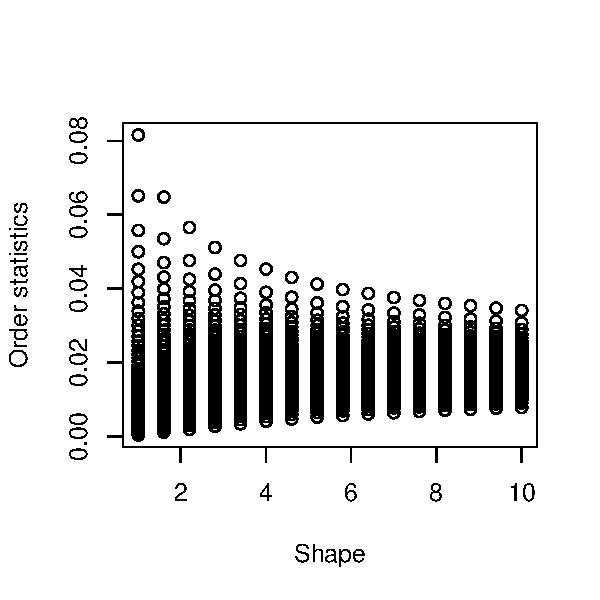
\includegraphics[scale=0.5]{plots/dirichlet}}
    \end{center}

    %The theoretical prior qualitatively matches the simulation.

   \end{column}
   \begin{column}{.40\textwidth}
   \begin{center}
  {\tiny $\| \Theta - \hat \Theta_\eta\|_\mathrm{F} / \| \Theta - \hat \Theta \|_\mathrm{F}$}
    \vspace{-0.5em}


\begin{figure}[h]
  \subfigure{%[$m/\mu = 0.2$; $s = 0$.]{
    \makebox{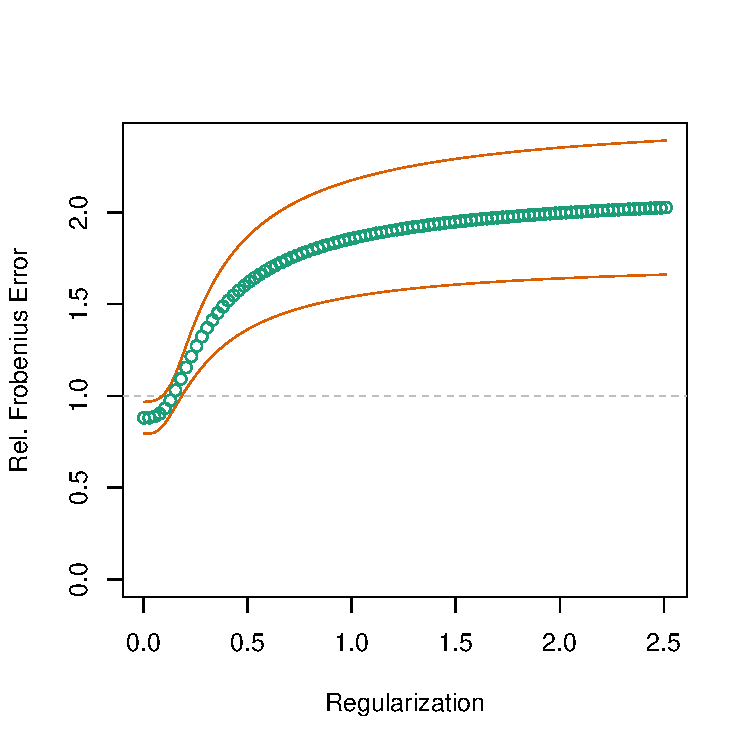
\includegraphics[scale=0.24]{plots/estimation-frob-s0-p020}}
  }
  \subfigure{%[$m/\mu = 1.0$; $s = 0$.]{
    \makebox{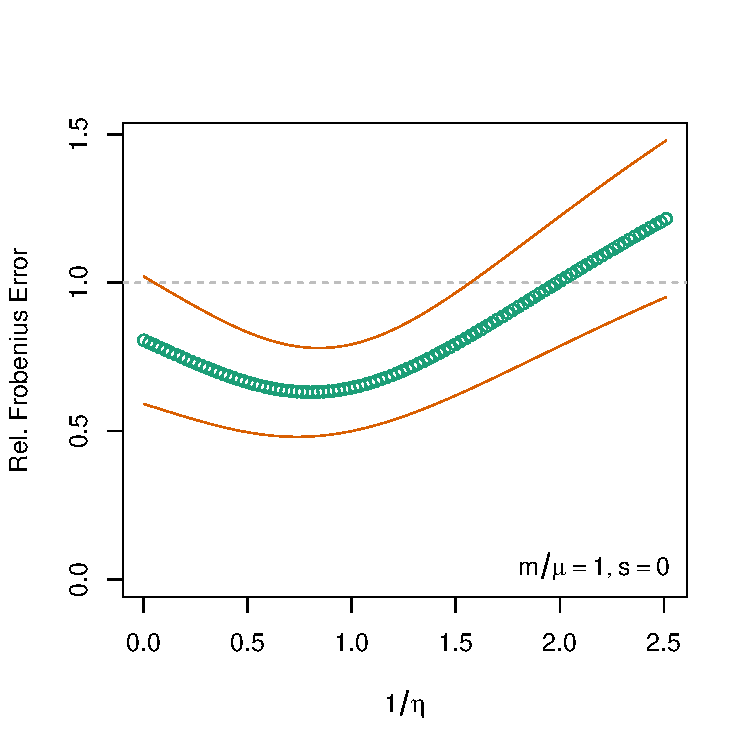
\includegraphics[scale=0.24]{plots/estimation-frob-s0-p100}}
  }
  \subfigure{%[$m/\mu = 2.0$; $s = 0$.]{
    \makebox{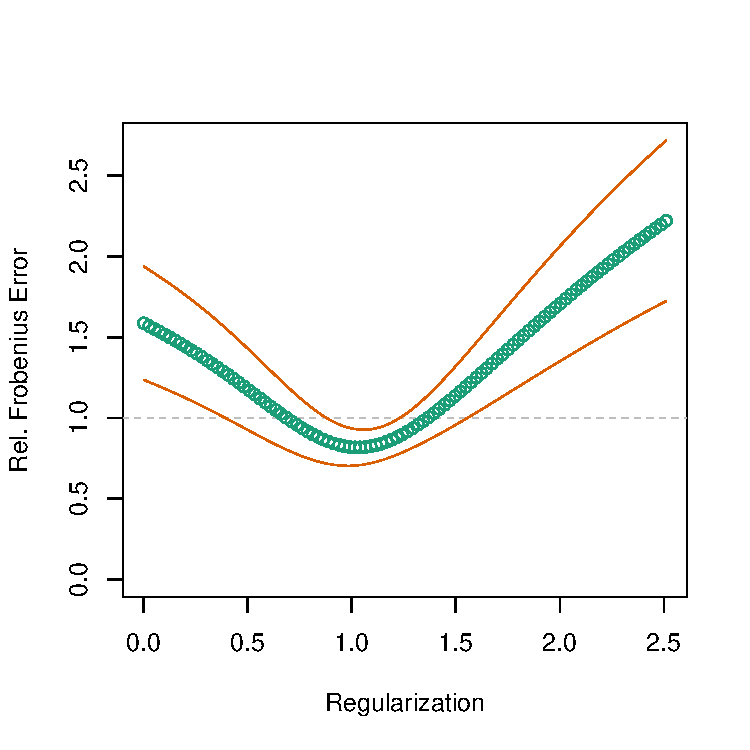
\includegraphics[scale=0.24]{plots/estimation-frob-s0-p200}}
  } \\
%\vspace{-2.0em}
  \subfigure{%[$m/\mu = 0.2$; $s = 4$.]{
    \makebox{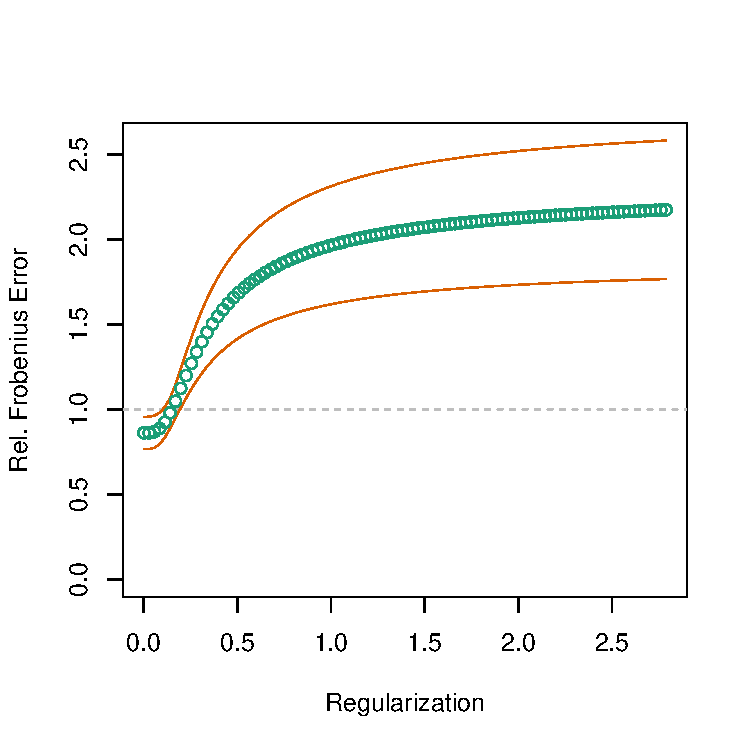
\includegraphics[scale=0.24]{plots/estimation-frob-p020}}
  }
  \subfigure{%[$m/\mu = 1.0$; $s = 4$.]{
    \makebox{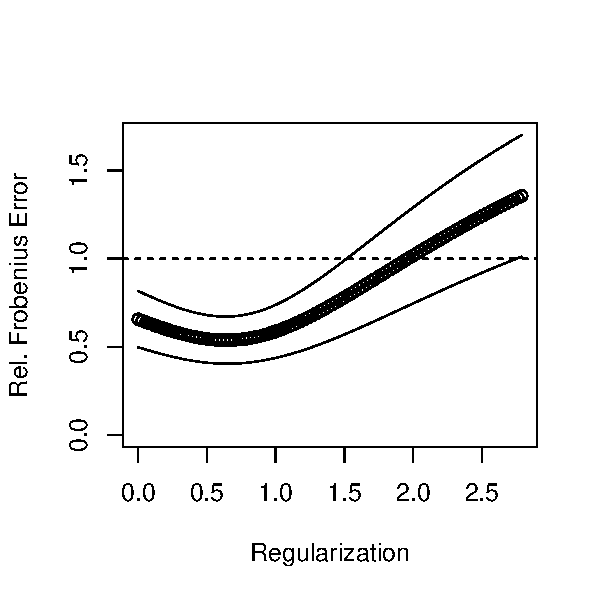
\includegraphics[scale=0.24]{plots/estimation-frob-p100}}
  }
  \subfigure{%[$m/\mu = 2.0$; $s = 4$.]{
    \makebox{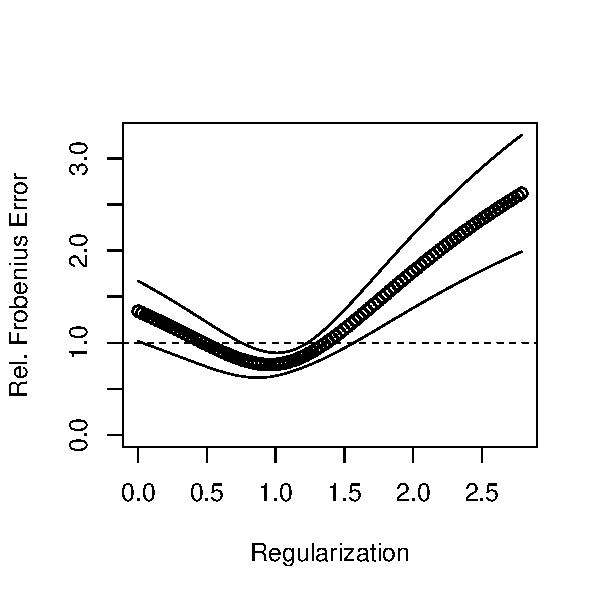
\includegraphics[scale=0.24]{plots/estimation-frob-p200}}
  } \\
%\vspace{-2.0em}
  \subfigure{%[$m/\mu = 0.2$; $s = 32$.]{
    \makebox{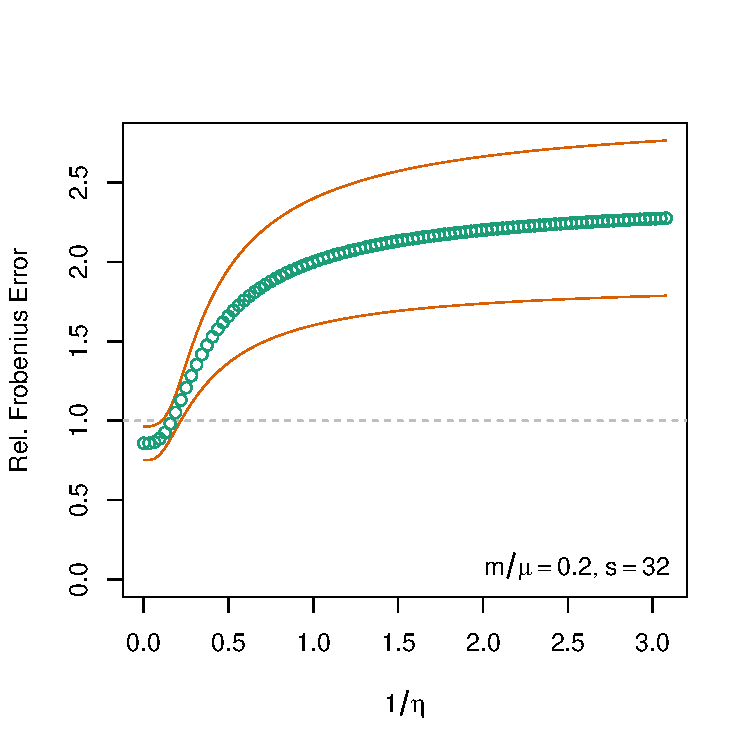
\includegraphics[scale=0.24]{plots/estimation-frob-s32-p020}}
  }
  \subfigure{%[$m/\mu = 1.0$; $s = 32$.]{
    \makebox{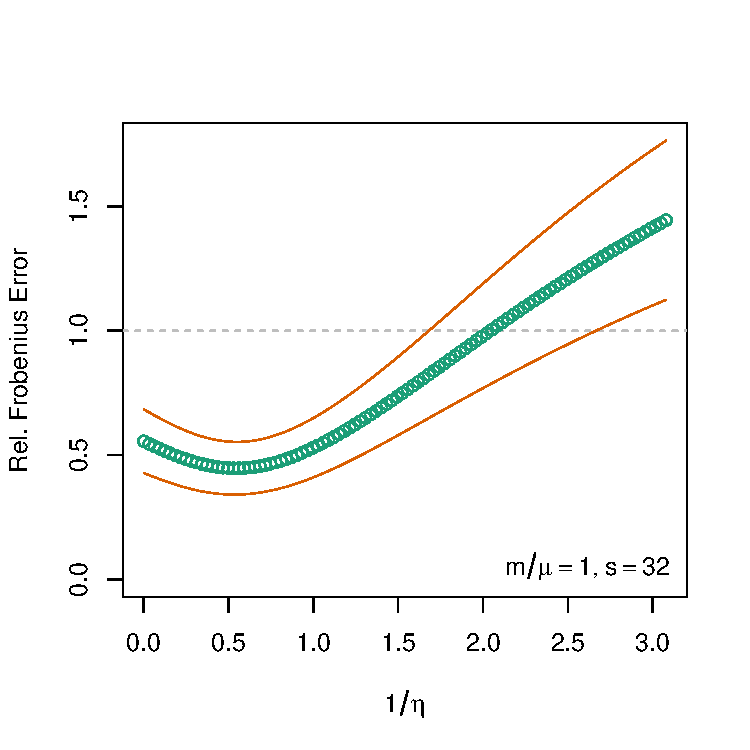
\includegraphics[scale=0.24]{plots/estimation-frob-s32-p100}}
  }
  \subfigure{%[$m/\mu = 2.0$; $s = 32$.]{
    \makebox{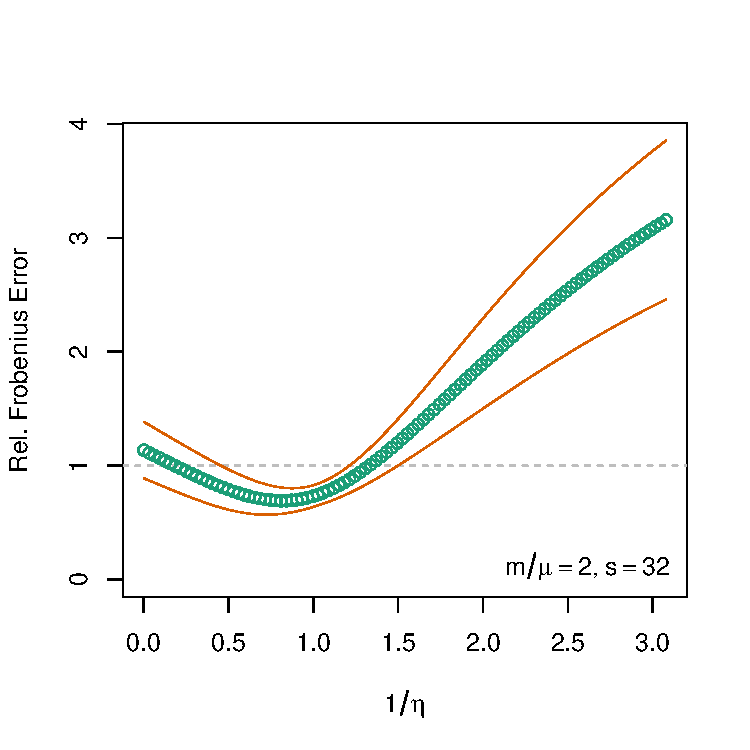
\includegraphics[scale=0.24]{plots/estimation-frob-s32-p200}}
  }
\setcounter{subfigure}{0}
%\vspace{-2.5em}
\end{figure}
  \end{center}
  %For certain values of $\eta$, the regularized estimate $\mathcal{\hat
  %L}_\eta$ outperforms the unregularized estimate $\mathcal{\hat L}$.

   \end{column}
   \begin{column}{.25\textwidth}
   \begin{center}
  {\tiny Optimal $\eta$ (empirical)}
    \vspace{-0.5em}
    \makebox{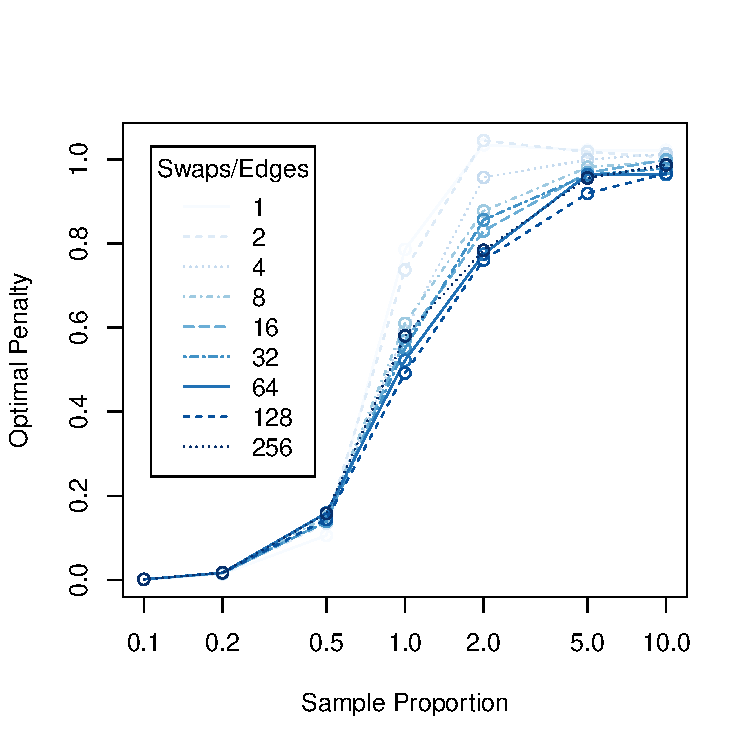
\includegraphics[scale=0.4]{plots/optimal}}

  {\tiny Optimal $\eta$ (theoretical)}
    \vspace{-0.5em}
    \makebox{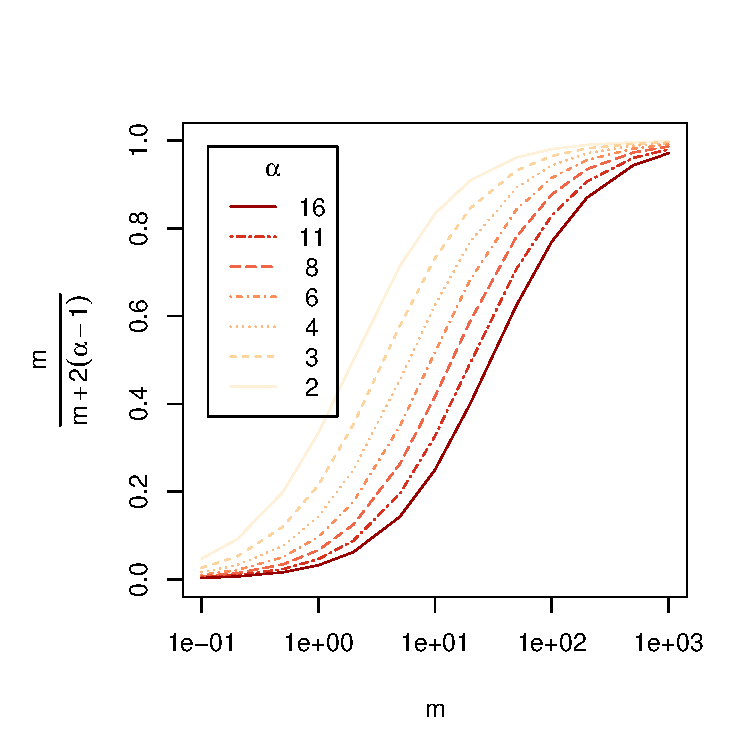
\includegraphics[scale=0.4]{plots/optimal-theory}}
    \vspace{1em}
  \end{center}

   %The behavior of the optimal $\eta$ agrees qualitatively with the theory.
   \end{column}
   \end{columns}

   \begin{columns}
   \begin{column}{.25\textwidth}
    The theoretical prior qualitatively matches the simulation. 
   \end{column}

   \begin{column}{.40\textwidth}
  For certain values of $\eta$, the regularized estimate $\mathcal{\hat
  L}_\eta$ outperforms the unregularized estimate $\mathcal{\hat L}$.
    \vfill
   \end{column}

   \begin{column}{.25\textwidth}
   The behavior of the optimal $\eta$ agrees qualitatively with the theory.
    \vfill
   \end{column}

   \end{columns}
            \end{block}

            \vfill

            \begin{block}{Conclusions}
\begin{itemize}
\item
We have
provided a statistical interpretation for the observation that popular 
diffusion-based procedures to compute a quick approximation to the first 
nontrivial eigenvector of a data graph Laplacian exactly solve a certain 
regularized version of the problem.
\item
We have
provided a statistical framework for regularized graph estimation, 
including providing a sampling model and applying Bayesian inference 
ideas directly to a graph Laplacian.
\item
We have
made explicit the implicit prior assumptions associated with making 
certain decisions (that are already made in practice) to speed up 
computations.
\end{itemize}

            \end{block}
          }
          % ---------------------------------------------------------%
          % end the column
        \end{minipage}
      \end{beamercolorbox}
    \end{column}
    % ---------------------------------------------------------%
    % end the column
  \end{columns}
  \vskip1ex
  %\tiny\hfill\textcolor{ta2gray}{Created with \LaTeX \texttt{beamerposter}  \url{http://www-i6.informatik.rwth-aachen.de/~dreuw/latexbeamerposter.php}}
  %\tiny\hfill{Created with \LaTeX \texttt{beamerposter}  \url{http://www-i6.informatik.rwth-aachen.de/~dreuw/latexbeamerposter.php} \hskip1em}
\end{frame}
\end{document}


%%%%%%%%%%%%%%%%%%%%%%%%%%%%%%%%%%%%%%%%%%%%%%%%%%%%%%%%%%%%%%%%%%%%%%%%%%%%%%%%%%%%%%%%%%%%%%%%%%%%
%%% Local Variables: 
%%% mode: latex
%%% TeX-PDF-mode: t
%%% End:
